\documentclass[conference]{IEEEtran}
\IEEEoverridecommandlockouts
\usepackage{cite}
\usepackage{amsmath,amssymb,amsfonts}
\usepackage{algorithmic}
\usepackage{graphicx}
\graphicspath{{../}}
\usepackage{textcomp}
\usepackage{xcolor}
\usepackage{booktabs}
\usepackage{multirow}
\usepackage{url}

% ---------------------------------------------------------------------------
% Revised draft (fixpaper.tex). Remaining open items are red \todo{} marks;
% each is explained in FIXPAPER_TODO.md.
% ---------------------------------------------------------------------------
\newif\ifshowtodos
\showtodostrue
\newcommand{\todo}[1]{\ifshowtodos\textcolor{red}{[TODO: #1]}\fi}
\newcommand{\verified}[1]{#1}  % wraps numbers already re-run and checked

\def\BibTeX{{\rm B\kern-.05em{\sc i\kern-.025em b}\kern-.08em
    T\kern-.1667em\lower.7ex\hbox{E}\kern-.125emX}}

\begin{document}

\title{Validated, yet Wrong: Four Ways Small-$n$ Metabolomics Machine Learning Passes Standard Checks\\
\thanks{Code, simulation, fixed analysis designs and verification scripts: \protect\url{https://github.com/Calvinkub/validated-yet-wrong} (tag \texttt{paper-v1}).}}

\author{
\IEEEauthorblockN{Chaiyaporn Orrudee}
\IEEEauthorblockA{\textit{Artificial Intelligence Technology, School of Information Technology} \\
\textit{King Mongkut's Institute of Technology Ladkrabang}\\
Bangkok, Thailand \\
67070217@kmitl.ac.th}
\and
\IEEEauthorblockN{Kanin Calvin Shomwiwat}
\IEEEauthorblockA{\textit{Artificial Intelligence Technology, School of Information Technology} \\
\textit{King Mongkut's Institute of Technology Ladkrabang}\\
Bangkok, Thailand \\
67070015@kmitl.ac.th}
}

\maketitle

% ===========================================================================
\begin{abstract}
Small-cohort metabolomics studies routinely support their headline scores with
cross-validation, permutation testing, and feature-attribution checks. We
audit four of our own earlier analyses of public NMR data and show four
failure modes in which a standard check passes while the reported result is
wrong or uninterpretable: (i) an outcome manufactured from the features
through change scores, (ii) putatively exogenous compounds that a
feature-removal faithfulness test ranks as highly as endogenous metabolites,
(iii) a label perfectly aliased with the sample-collection protocol, and
(iv) a label whose name does not match what it encodes. For each, we give the
check it passes and a targeted control that exposes it. In a bariatric-surgery
responder forecast, a label-permutation test with refitting gave
$p=\verified{0.001}$, yet the model scored below a learn-nothing baseline, and
after correcting the outcome the trained model (PR-AUC \verified{0.554}) was
still no better than that baseline (\verified{0.589}).
In simulation with no forecastable individual response, label permutation
rejected in 11--100\% of datasets at $\alpha=0.05$, rising with sample size;
residualising change on each marker's own baseline still rejected in
8--29\%, whereas residualising on all baselines jointly held the rate at
5--8\%, slightly above nominal. We release the controls as a reusable
checklist with reference code.
\end{abstract}

\begin{IEEEkeywords}
metabolomics, NMR, validation, data leakage, regression to the mean,
permutation test, feature attribution, confounding, reproducibility
\end{IEEEkeywords}

% ===========================================================================
\section{Introduction}
\label{sec:intro}

Machine-learning studies on small metabolomics cohorts ($n<200$) can report
near-perfect discrimination, and readers are asked to trust these numbers
because the authors used cross-validation, a permutation test, and an
explanation method such as SHAP \cite{lundberg2017}. Yet leakage and related
evaluation errors have been documented across hundreds of ML-based studies in
many fields \cite{kapoor2023}, and omics data add hazards of their own:
acquisition batch, sample handling, and repeated measurements of the same
person \cite{leek2010}. With a few dozen subjects, any of these can produce a
near-perfect score.

Each of these checks answers a narrow question. Cross-validation asks whether
the model generalises to new samples \emph{drawn the same way}; a label
permutation asks whether the features carry \emph{any} association with the
label; a faithfulness test asks whether the model \emph{relies} on a feature.
None asks whether the label measures what it claims to, or whether the
association is biological. A result can therefore pass any one of these checks
and still be wrong.

The four analyses we examine are our own earlier work: a responder forecast
and a feature-attribution study on MTBLS242, and a diabetes classifier on
MTBLS1 \cite{bridge2026, roar2026, honest2026}. Each passed the checks we
had applied at the time. This paper makes four contributions:
\begin{enumerate}
  \item A taxonomy of four failure modes, each paired with the standard check
        it passes and a targeted control that catches it
        (Table~\ref{tab:taxonomy}).
  \item A \emph{pairing-destroyed null} for change-score outcomes, a
        conservative diagnostic for outcomes manufactured by regression to
        the mean.
  \item A simulation study (36{,}000 datasets) showing that label permutation
        becomes \emph{more} wrong as $n$ grows, that the common per-marker
        regression-to-the-mean correction is itself liberal for correlated
        markers, and that joint residualisation brings the error rate close
        to nominal.
  \item An open checklist and reference implementations of the controls for
        metabolomics ML studies.
\end{enumerate}

% ===========================================================================
\section{Related Work}
\label{sec:related}

\subsection{Regression to the mean and mathematical coupling}
Correlating change with initial value is a known statistical artefact
\cite{oldham1962, tu2007, barnett2005}, and a change score that shares terms
with the baseline is mathematically coupled to it \cite{archie1981}:
measurement error and within-person variation make extreme baselines move
back toward the mean, so baseline ``predicts'' change even when nothing
happens. The epidemiological remedies (analysis of covariance, Oldham's
method) are well known \cite{vickers2001, glymour2005}. Our contribution is
not the artefact but its interaction with ML practice: an outcome
\emph{defined} from change scores, a flexible model given the baselines as
features, and a label permutation as the significance test. We show that this
combination certifies the artefact, and that the per-marker correction a
careful analyst might add is not sufficient.

\subsection{Leakage and confounding in ML-based science}
Kapoor and Narayanan \cite{kapoor2023} catalogue leakage types, including
features that act as proxies for the outcome and non-independence between
training and test data. Batch effects can be perfectly confounded with the
biological variable of interest, in which case no analysis can separate them
\cite{leek2010}; analytical and pre-analytical bias in serum metabolomics is
well documented \cite{teahan2006, han2022, bernini2011}, and exogenous
compounds introduced during sampling can appear in NMR spectra
\cite{vandersar2015}. Reporting guidelines such as TRIPOD+AI
\cite{collins2024} require that the outcome definition and its relation to
the predictors be stated. Our cases are concrete metabolomics instances of
these categories, each paired with a test that detects it.

\subsection{Feature-attribution faithfulness}
SHAP \cite{lundberg2017} attributes a prediction to features; ROAR
\cite{hooker2019} tests whether the attributed features matter by removing
them and retraining. Both answer a question about the \emph{model}, and
attribution methods can mislead even about model behaviour
\cite{adebayo2018, kumar2020}. ROAR was not designed to say whether a feature
is biological, but a low ROAR curve is easily read as confirming that the
top-ranked metabolites are meaningful. We use putatively exogenous compounds
and a synthetic artefact to show why that reading is unsafe.

\subsection{Permutation tests for classifiers}
A label permutation tests the null hypothesis that features and labels are
independent \cite{ojala2010}. Rejecting it shows only that \emph{some}
association exists. If the label is computed from the features, that
association is guaranteed, and the test answers a question nobody asked.
The permutation must also refit the model on every permuted label vector:
permuting labels against fixed out-of-fold scores is not a valid test
(Section~\ref{sec:sim}); the broader fragility of resampling-based
validation on small cohorts is well established
\cite{westerhuis2008, broadhurst2006, varma2006, varoquaux2018}.

% ===========================================================================
\section{Data and Common Setup}
\label{sec:data}

\subsection{Datasets}
\textbf{MTBLS242} \cite{mtbls242, gralka2015}: serum $^1$H-NMR from a
bariatric surgery cohort, released 10 Feb.\ 2017. The sample sheet lists 465
samples at five visits, labelled in its time-point factor as preoperative
(106), and 3, 6, 9 and 12 months after surgery (98, 98, 92 and 71);
21 metabolites are quantified. We re-downloaded the sheet from MetaboLights
on 15 Oct.\ 2026 and it is byte-identical to the copy used in all
experiments. Patient identifiers are not a column; they are recoverable from
sample names with the pattern \verb|^(\d+)[-_](\d+)[-_]S$| (one 6-month
sample, \verb|2_0242_2|, does not match and does not affect any analysis
here, which uses only the preoperative and 12-month visits). All 71
twelve-month patients also have a preoperative sample. The sheet records
neither the surgical procedure per sample nor any clinical covariate such as
body-mass index, although the study design lists both gastric bypass and
sleeve gastrectomy.

\textbf{MTBLS1} \cite{salek2007}: urine $^1$H-NMR, type 2 diabetes vs.\
control; 132 samples from 40--42 subjects (12 volunteers sampled at seven
time points; 28--30 patients whose sample-to-patient membership is not
deposited; see Section~\ref{sec:case3}).

\textbf{MTBLS881} \cite{maltesen2020}: serum $^1$H-NMR from 50 adults
undergoing cardiac surgery with cardiopulmonary bypass, sampled at six times
(from $-1$ to 20\,h) from two sites (left atrium, LA; pulmonary artery, PA).
We use it only to replicate Case~1 on a second cohort: 47 patients have both
the $-1$\,h and 20\,h samples at each site.

\subsection{Models and evaluation}
We deliberately reuse the models from the original analyses rather than
tuning new ones, since the point is to evaluate the checks, not the models.
Cases 2 and 3 use XGBoost \cite{chen2016} with monotonic constraints whose
directions were assigned from the metabolomics literature; Case~4 re-runs the
unconstrained XGBoost of its original analysis. Case~1 uses
L2-penalised logistic regression with literature-assigned sign constraints
on the marker coefficients; its replication (Case~1b) uses the same model
without constraints. The headline metric is PR-AUC (average precision),
reported next to the prevalence it must beat. Cross-validation is repeated
and grouped by subject wherever subjects can be identified. Every analysis of
Case~1 includes a learn-nothing baseline: a fixed, unfitted score that any
trained model must beat, with intervals from bootstrap resampling of
subjects.

\begin{table*}[t]
\centering
\caption{Four failure modes: the standard check each passes and the control
that exposes it. ``Reported result'' is the score of our original analysis.}
\label{tab:taxonomy}
\footnotesize
\begin{tabular}{@{}c p{3.4cm} l l p{3.2cm} p{3.2cm}@{}}
\toprule
Case & Failure mode & Data & Reported result & Standard check passed & Exposing control \\
\midrule
1 & Outcome manufactured from features & MTBLS242 & PR-AUC 0.683 & Label permutation (refit), $p=0.001$ & Learn-nothing baseline; joint residualisation \\
2 & Putative contaminants ranked with biology & MTBLS242 & PR-AUC 0.973 & ROAR faithfulness & Known-artefact positive control \\
3 & Collection protocol equals label & MTBLS1 & PR-AUC 0.976 & Subject-grouped CV & Metadata and protocol audit \\
4 & Label name $\neq$ label meaning & MTBLS242 & ROC-AUC 0.973 & Subject-grouped CV & Label-provenance audit \\
\bottomrule
\end{tabular}
\end{table*}

% ===========================================================================
\section{Case 1: An Outcome Manufactured from the Features}
\label{sec:case1}

\subsection{Setup}
Task: predict from the preoperative profile whether a patient is a
twelve-month ``strong responder,'' defined as $\geq$9 of 11 markers changing
in the expected direction. 71 paired patients, 31 responders.

\subsection{Why the standard check passes}
Baseline $x_0$ is both the predictor and a term in the outcome
$\Delta = x_{12} - x_0$. Under pure noise, $\operatorname{corr}(x_0, \Delta)<0$
by construction; the observed median was \verified{$-0.62$}. A label
permutation breaks the label--feature link entirely, so it tests against a
null that the coupled outcome trivially beats.

\subsection{Exposing controls}
\textbf{Learn-nothing baseline.} A fixed score built from the baselines and
the expected marker directions, with no fitting, exploits regression to the
mean as well as any trained model can. A trained model that does not beat it
has learned nothing beyond the coupling.

\textbf{Pairing-destroyed null.} Shuffle which twelve-month sample belongs
to which subject, recompute the outcome from scratch, and rescore. This keeps
the arithmetic coupling and removes any real individual-level signal. Because
shuffling breaks the positive correlation between visits, the null has
\emph{stronger} coupling than the observed data, so its lift is expected to
exceed the observed lift even when a real response exists
(Section~\ref{sec:sim}). It is therefore a one-sided diagnostic: a model that
\emph{clears} it has shown something beyond regression to the mean; a model
that does not clear it has shown nothing either way.

\textbf{Joint residualisation.} Inside each training fold, regress each
marker's change on all 11 baselines and define the label from the residuals.
Section~\ref{sec:sim} shows that this, unlike per-marker residualisation,
keeps the false-positive rate close to nominal.

\subsection{Result}
\textbf{Original design} (raw change, $\geq$9 of 11 markers, putative
contaminants included). The trained model reaches PR-AUC \verified{0.683}
against a prevalence of \verified{0.437} (our originally reported
\verified{0.671} does not reproduce exactly on re-run). A label permutation
with the model refitted on every permutation (1{,}000 permutations) gives
$p=\verified{0.001}$, the floor. Yet the learn-nothing scorer reaches
\verified{0.709}, above the model (gap \verified{$-0.025$}, repeat-level
interval [\verified{$-0.047$}, \verified{$-0.006$}]). Consistent with this,
the observed lift (\verified{1.57$\times$}) does not clear the
pairing-destroyed null (median \verified{2.04$\times$}; Fig.~\ref{fig:case1}),
and refitting the full model on each shuffle gives the same picture (median
\verified{1.99$\times$}, 500 replicates). The permutation test certifies a
model that does not beat an unfitted score.

\textbf{Corrected designs} (change residualised inside each training fold,
contaminants removed). Table~\ref{tab:case1} shows the per-marker design of
the original repository and the joint design recommended by
Section~\ref{sec:sim}. In both, the trained model does not beat the
learn-nothing scorer, and the subject-bootstrap interval for the gap spans
zero. The refitted permutation test also finds nothing, but its null sits
\emph{above} the observed statistic in every replicate ($p=1.0$), which a
well-calibrated null would rarely do. A plausible cause, which we did not
test, is that the sign constraints force a literature-signed score even on
permuted labels. We therefore do not read $p=1.0$ as a calibrated $p$-value.
The defensible statement is that the model is \emph{no better than} the
scorer; at $n=71$ the interval cannot exclude a modest real gain.

\begin{table}[t]
\centering
\caption{Case 1, corrected designs. PR-AUC values are means over 20 repeats
of the per-fold average precision. Gap = model $-$ learn-nothing scorer,
computed on held-out predictions pooled within each repeat, which is why it
differs slightly from the difference of the PR-AUC rows; interval from a
bootstrap over the 71 subjects. Prevalence differs because the joint design
yields a different responder count, so compare lifts and gaps, not PR-AUC
levels.}
\label{tab:case1}
\footnotesize
\begin{tabular}{@{}lrr@{}}
\toprule
 & Per-marker resid. & Joint resid. \\
\midrule
Responders / 71          & 31 & 37 \\
Prevalence               & 0.437 & 0.521 \\
Model PR-AUC             & 0.483 & 0.554 \\
Learn-nothing PR-AUC     & 0.522 & 0.589 \\
Gap (pooled)             & $-0.042$ & $-0.037$ \\
95\% interval            & [$-0.149$, $+0.052$] & [$-0.111$, $+0.037$] \\
Refit permutation $p$ (B) & 1.000 (200) & 1.000 (1000) \\
Model lift               & 1.11 & 1.06 \\
Pairing-null lift, median & 1.04 & 1.05 \\
\bottomrule
\end{tabular}
\end{table}

\begin{figure}[t]
\centering
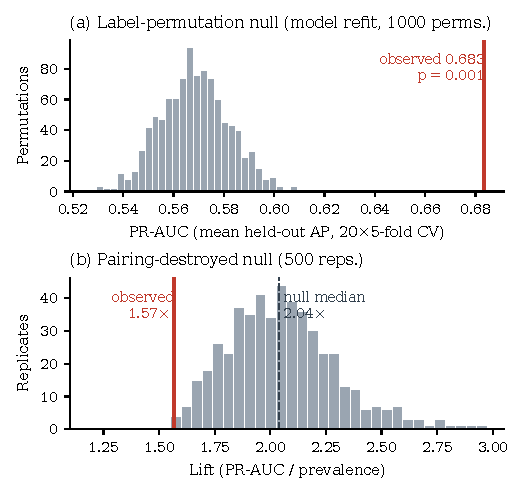
\includegraphics[width=\columnwidth]{figures/case1_nulls.pdf}
\caption{Original (withdrawn) design. (a) Label-permutation null of
average precision, model refitted per permutation. (b) Pairing-destroyed null
of lift. The label permutation rejects. The pairing-destroyed null sits above
the observed model, which is expected by construction
(Section~\ref{sec:sim}) and means only that the model has not shown anything
beyond regression to the mean.}
\label{fig:case1}
\end{figure}

\subsection{Replication on a second cohort}
We repeated the four tests on MTBLS881 with the design fixed in a
pre-registration file before any model was fitted: baseline $-1$\,h versus
20\,h; both sites analysed separately (LA declared primary); 11 marker
metabolites chosen in advance; improvement direction taken from training-fold
mean change only; $K$ chosen so prevalence is near 0.5; exogenous drugs
(propofol, heparin, ethanol) excluded. The model is unconstrained ridge
logistic regression with the same repeated CV as Case~1. One deviation from
the pre-registration: after a single timing run, which printed $K$,
prevalence and PR-AUC for one site, we reduced the number of null replicates
for run time (300 permutations for the main designs, 200 for the
exogenous-compound variant, 150 refitted pairing replicates); designs,
markers and the $K$ rule were not changed. This is a different, acute setting
(hours after surgery, not a year), so it tests the statistical artefact, not
the surgical biology. With 47 patients every interval is wide
(Table~\ref{tab:case1b}).

\textbf{Raw change replicates.} At both sites a label permutation rejects
($p=\verified{0.007}$), yet the model does not beat the learn-nothing scorer
(pooled gap \verified{$-0.037$} and \verified{$+0.013$}, both intervals
spanning zero), and the pairing-destroyed null reaches equal or higher lift
(median \verified{1.49} and \verified{1.40} vs.\ observed \verified{1.29} and
\verified{1.19}). Refitting the full model on each shuffle puts the observed
lift inside the null ($p=\verified{0.86}$ at LA, \verified{0.91} at PA).

\textbf{Residualised outcomes replicate only partly.} At PA, joint
residualisation shows no signal ($p=\verified{0.977}$), matching MTBLS242. At
LA the per-marker outcome is permutation-significant ($p=\verified{0.003}$),
which the simulation predicts can happen without real signal. For LA joint
residualisation the permutation test is not significant
($p=\verified{0.103}$) while the model's lift (\verified{1.45}) exceeds the
scorer-based pairing-null 95th percentile (\verified{1.27}). The tests
disagree here, and 47 patients cannot resolve it. Every gap interval in
Table~\ref{tab:case1b} includes zero.

\textbf{Exogenous compounds create apparent signal.} In a variant that adds
propofol, heparin and ethanol both as features and as markers (14 markers,
so the $K$ rule now selects $K=8$ for the joint outcome), the
joint-residualised outcome becomes permutation-significant at both sites
($p=\verified{0.005}$, the floor for 200 permutations), against
$p=\verified{0.103}$ and \verified{0.977} without them. At LA the gap also
becomes \verified{$+0.163$} [\verified{$+0.069$}, \verified{$+0.252$}], the
only interval in this replication that excludes zero; at PA the gap stays
near zero (\verified{$+0.008$}). Because the variant changes both the
features and the label definition, it does not isolate a mechanism, but the
pattern matches Case~2: drugs administered during surgery can distinguish
samples for reasons unrelated to the response being modelled.

\begin{table*}[t]
\centering
\caption{Case 1 replication on MTBLS881 ($n=47$ per site). PR-AUC columns are
means of per-fold average precision; Gap = model $-$ learn-nothing scorer on
held-out predictions pooled within each repeat, so it is not the difference
of the two PR-AUC columns; interval from a subject bootstrap. $K$ = number of
the 11 markers required to define a responder.}
\label{tab:case1b}
\footnotesize
\begin{tabular}{llrrrrrrr}
\toprule
Site & Outcome & Prev. & PR-AUC & Scorer & Gap [95\% CI] & $p_{\mathrm{perm}}$ & Lift & Pair-null lift \\
 & & & & PR-AUC & (pooled) & (refit) & & med. (p95) \\
\midrule
LA & Raw change ($K{=}10$) & 0.49 & 0.632 & 0.695 & $-0.037$ [$-0.231$, $+0.118$] & 0.007 & 1.29 & 1.49 (2.09) \\
LA & Per-marker resid. ($K{=}6$) & 0.55 & 0.678 & 0.542 & $+0.164$ [$-0.004$, $+0.309$] & 0.003 & 1.23 & 1.05 (1.25) \\
LA & Joint resid. ($K{=}6$) & 0.43 & 0.619 & 0.545 & $+0.071$ [$-0.077$, $+0.190$] & 0.103 & 1.45 & 1.06 (1.27) \\
\midrule
PA & Raw change ($K{=}10$) & 0.64 & 0.757 & 0.723 & $+0.013$ [$-0.111$, $+0.154$] & 0.007 & 1.19 & 1.40 (1.89) \\
PA & Per-marker resid. ($K{=}6$) & 0.51 & 0.631 & 0.546 & $+0.078$ [$-0.086$, $+0.222$] & 0.096 & 1.24 & 1.05 (1.27) \\
PA & Joint resid. ($K{=}6$) & 0.53 & 0.598 & 0.629 & $-0.034$ [$-0.169$, $+0.092$] & 0.977 & 1.12 & 1.06 (1.23) \\
\bottomrule
\end{tabular}
\end{table*}

% ===========================================================================
\section{Case 2: Putative Contaminants Ranked with Biology}
\label{sec:case2}

\subsection{Setup}
ROAR \cite{hooker2019} removes the top-$k$ attributed features, retrains, and
compares the score with removing $k$ random features. Here the attribution is
SHAP on the MTBLS242 pre- vs.\ 12-month task (177 samples, 21 metabolites).
We repeat our original analysis with three fixes: cross-validation is grouped
by patient (10 repeats of 5 folds), attribution is recomputed after every
retrain (recursive ROAR), and the random null uses 500 distinct draws per $k$
(exhaustive for $k\leq 2$) under the same folds as the informed runs.
Grouped baseline PR-AUC is \verified{0.973}; ungrouped CV gives
\verified{0.972}.

\subsection{Why the standard check passes}
Recursive ROAR removes, in order, dimethyl sulfone, isopropanol, L-valine,
glycine, methanol, and then further metabolites. From $k=3$ onward the
curve lies below almost the entire random band (null percentile
\verified{0.0--0.2}), so ROAR reports that the removed features genuinely
matter to the model. That is true. But isopropanol and methanol are not
expected products of human metabolism at these levels; isopropanol is used
for skin preparation, and both can enter samples during collection and
handling \cite{bernini2011, vandersar2015}. Dimethyl sulfone is less clear:
it is a regular low-micromolar plasma metabolite that derives from diet,
intestinal bacterial metabolism and endogenous methanethiol metabolism
\cite{engelke2005}, and diet and gut flora may change after bariatric surgery.
We therefore call the three compounds \emph{putatively exogenous}, with the
weakest case for dimethyl sulfone. Their identity as handling artefacts is not
established from the deposited data, and the argument below does not depend
on it.

\subsection{Exposing control: artefact vs.\ biology}
At $k=3$, removing the putatively exogenous trio gives PR-AUC
\verified{0.954} (null percentile \verified{0.2}); removing three endogenous
markers (lipoproteins, L-valine, L-tyrosine) gives \verified{0.959}
(percentile \verified{1.2}). The \verified{0.006} gap is far smaller than the
fold standard deviation of about \verified{0.03}. ROAR treats the two groups
alike.

A spiked positive control makes the point without relying on the identity of
any real compound. We add a synthetic feature $d\,y + \mathcal{N}(0,1)$,
which depends only on the label and carries no biology, and measure both its
SHAP rank and the drop in PR-AUC when it alone is removed and the model
retrained (10 draws per $d$, Table~\ref{tab:spike}). At $d=1.75$, an effect
size similar to dimethyl sulfone's, the spike is ranked first by both, and
removing it costs more than removing any real metabolite (\verified{0.0127}
vs.\ \verified{0.0073} for dimethyl sulfone). Removal-based importance ranks
a feature by how much non-redundant signal it carries, whatever its origin;
a low ROAR curve cannot by itself support a biological reading of the
top-ranked features.

\begin{table}[t]
\centering
\caption{Spiked artefact: median rank among 22 features (1 = most
important). Removal rank orders features by the PR-AUC drop when each is
removed alone and the model retrained.}
\label{tab:spike}
\footnotesize
\begin{tabular}{@{}rrr@{}}
\toprule
$d$ & SHAP rank & Removal rank \\
\midrule
0.75 & 10 & 14.5 \\
1.25 & 3 & 3 \\
1.75 & 1 & 1 \\
\bottomrule
\end{tabular}
\end{table}

\begin{figure}[t]
\centering
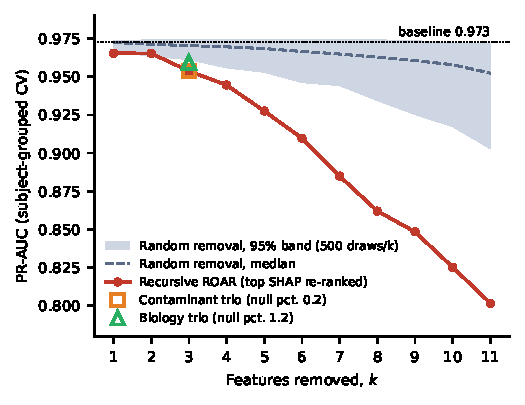
\includegraphics[width=\columnwidth]{figures/case2_roar.pdf}
\caption{Recursive ROAR on MTBLS242 against 500-draw random-removal bands.
The informed curve lies below the band from $k=3$ onward whether the removed
features are putatively exogenous or endogenous.}
\label{fig:case2}
\end{figure}

\subsection{Caveats}
This is one cohort, and its label is confounded with surgery (Case~4).
Random draws overlap and share folds, so percentiles below the band mean
``outside the random range,'' not calibrated $p$-values. Attribution used
all 177 samples, which makes informed removal slightly optimistic. The
multi-seed ranking places L-valine above lipoproteins, the reverse of the
original ranking; we kept the original endogenous trio for comparability.
Both trios were chosen after the original analysis, not in advance.

% ===========================================================================
\section{Case 3: Collection Protocol Equals Label}
\label{sec:case3}
\subsection{Setup}
The Case~3 model is our original monotonic XGBoost on 132 urine spectra,
evaluated by CV grouped by subject. With seed 42 it reproduces our reported
PR-AUC of \verified{0.976}; over 20 CV seeds the mean is \verified{0.911}
(range \verified{0.845--0.975}), so the headline was a favourable split.

\subsection{Why the standard check passes}
Subject-grouped CV prevents the same person from appearing in training and
test folds. It cannot detect a confound shared by every member of a class.

\subsection{Exposing control: metadata and protocol audit}
We cross-tabulated the label against all 64 columns of the deposited sample
and assay sheets. Of these, 56 are constant (instrument, probe, pulse
sequence, temperature) and six are per-sample identifiers or file paths;
apart from the label, only sex varies. There is no date, run, rack or
acquisition-order column. The acquisition parameters in the 132 nmrML headers
are likewise constant except for per-sample calibrations (pulse width,
phasing, referencing), none of which defines sessions that span both classes;
pulse width alone separates the classes with ROC-AUC \verified{0.77}, which
may reflect urine composition or acquisition session and cannot be resolved.

The deposited protocol, however, describes two different studies. Controls
were 12 volunteers aged 18--55 with BMI 19--30, each sampled at seven fixed
time points; patients were aged 30--65 with BMI 25--40 and sampled one to
three times. Every control sample name begins with \verb|ADG19007u| and
every diabetic sample name with \verb|ADG10003u| (Table~\ref{tab:case3}),
consistent with separate collection protocols. Age, BMI, sampling schedule,
and any difference in collection, storage or diet protocol are therefore
aliased with the label, and none is recorded per sample. No within-protocol
comparison is possible because each protocol contains one class. The sample
prefix itself is only a marker of this design (a logistic model given the
prefix scores PR-AUC \verified{1.000} under the same CV, as any perfect
label proxy would); the problem is the design it reveals.

Sex is imbalanced (controls \verified{66.7\%} male vs.\ cases
\verified{45.8\%} of samples) but not confounded. Subject identity is not
deposited: the control numbering yields exactly 12 volunteers, matching the
protocol, while the 48 diabetic samples come from 28--30 patients whose
sample-to-patient membership cannot be recovered. A numbering heuristic used
in our original analysis merged at least three pairs of distinct patients.
Merging errs toward conservative CV, and ungrouped CV (\verified{0.969})
differs little, so grouping does not drive the result; the design does, and
it cannot be removed by any analysis of these data.

\begin{table}[t]
\centering
\caption{MTBLS1 samples by label, sample-name prefix and sex. The prefix
determines the label exactly; sex does not.}
\label{tab:case3}
\footnotesize
\begin{tabular}{@{}llrrrr@{}}
\toprule
Label & Prefix & F & M & Samples & Subjects \\
\midrule
Control & \texttt{ADG19007u} & 28 & 56 & 84 & 12 \\
T2DM    & \texttt{ADG10003u} & 26 & 22 & 48 & 28--30 \\
\midrule
Total   &                    & 54 & 78 & 132 & 40--42 \\
\bottomrule
\end{tabular}
\end{table}

% ===========================================================================
\section{Case 4: The Label Is Not What It Is Called}
\label{sec:case4}
Our ``obese vs.\ non-obese'' task on MTBLS242 is in fact ``preoperative vs.\
twelve months after surgery'': \verified{71} of \verified{106} patients
appear in both classes, so the label records the visit, not a measurement of
obesity. The originally reported ROC-AUC of 0.973 came from a single
stratified 5-fold split (re-run: \verified{0.974}). Over 10 repeats of 5-fold
CV with the same model, subject-grouped and naive CV both give ROC-AUC
\verified{0.965}, although in naive CV \verified{65\%} of test samples
have the same patient's other visit in the training folds. Removing that
leakage does not lower the score, so the issue is not leakage but label
meaning. The sample sheet records no body-mass
index, so whether any twelve-month patient is in fact non-obese cannot be
checked; a year after bariatric surgery many patients need not be.

A classifier trained on this label learns everything that differs between a
patient before surgery and the same patient a year later: weight loss, but
also post-surgical diet, supplements and medication, fasting state, and the
year-long gap in sample storage. Its score is not evidence that the serum
profile identifies obesity in a general population, where lean and obese
people differ in age, sex and lifestyle rather than in surgical history. The
correct description is ``pre- vs.\ post-bariatric-surgery classification,''
and the check that exposes the mismatch is not statistical: write down, in one
sentence, what physically distinguishes the two classes.

% ===========================================================================
\section{Simulation Study}
\label{sec:sim}

\subsection{Design}
Each subject $i$ has a persistent level $\mu_{ij}$ for $p=11$ outcome markers,
with a shared factor (inter-marker correlation $\rho=0.3$), and ten auxiliary
features $z_i\sim\mathcal{N}(0,I)$. Observed visits are
\begin{align}
x^{(0)}_{ij} &= \sqrt{r}\,\mu_{ij} + \sqrt{1-r}\,\varepsilon^{(0)}_{ij},\\
x^{(12)}_{ij} &= \sqrt{r}\,(\mu_{ij} + \gamma\, g_i\, s_j) + \sqrt{1-r}\,\varepsilon^{(12)}_{ij},
\end{align}
where $r$ is the reliability (share of variance that persists between
visits), $s_j\in\{\pm1\}$ the expected direction of marker $j$, and
$g_i = w^\top z_i/\lVert w\rVert$ a forecastable response propensity. With
$\gamma=0$ no individual response exists, so any association between baseline
and outcome is regression to the mean. The outcome is the MTBLS242-style rule
``$\geq$6 of 11 markers change in the expected direction.'' The model is
ridge regression ($\lambda=10$) on the 21 standardised baseline features,
scored out-of-fold in 5-fold CV by average precision.

We vary $n\in\{50,100,200,500\}$, $r\in\{0.25,0.5,0.75\}$ and
$\gamma\in\{0,0.25,0.5\}$, with 1{,}000 datasets per cell. Setting $r=0.25$
reproduces the median baseline--change correlation of $-0.62$ observed in
MTBLS242. Each dataset is tested four ways at $\alpha=0.05$, each with 200
null replicates and the model refitted on every replicate:
\begin{enumerate}
  \item \textbf{Label permutation} on the raw-change outcome.
  \item \textbf{Pairing-destroyed null} on lift (AP over prevalence).
  \item \textbf{Per-marker residualisation}: within each training fold,
        regress change$_j$ on baseline$_j$; label from residuals; permute.
  \item \textbf{Joint residualisation}: as (3), but regress change$_j$ on all
        11 baselines.
\end{enumerate}
A permutation test that holds out-of-fold scores fixed and permutes only the
labels rejected 9.7\% of pure-noise datasets in our sanity check; refitting
on each permutation \cite{ojala2010} gave 5.3\%, so all tests refit.

\subsection{Results}
Table~\ref{tab:sim} and Fig.~\ref{fig:sim} give the rejection rates.

\textbf{Label permutation is wrong, and more so with more data.} With no
individual response, it rejected in 26\% of datasets at $n=50$ and 100\% at
$n=500$ when $r=0.25$; even at $r=0.75$ it reached 90\% at $n=500$.
More subjects estimate the regression-to-the-mean artefact more precisely;
they do not remove it.

\textbf{Per-marker residualisation is not enough.} Residualising each
marker's change on its own baseline left false-positive rates of 8--29\%,
again rising with $n$. When markers are correlated, residual change in
marker $j$ remains correlated with the baselines of the other markers,
which the model also sees.

\textbf{Joint residualisation is close to nominal but slightly liberal.}
Regressing each change on all baselines kept the rate between 5.3\% and
8.1\%, without a trend in $n$; in most cells the Wilson interval lies just
above 5\%, so a small excess remains. Its power when a real response exists
is close to that of per-marker residualisation (e.g.\ 97.5\% vs.\ 97.0\% at
$\gamma=0.25$, $r=0.25$, $n=500$), but it is low at small $n$ and low
reliability (19\% at $n=50$ in the same setting).

\textbf{The pairing-destroyed null is valid but conservative.} Its
false-positive rate never exceeded 4.3\%, but at the MTBLS242-like reliability
$r=0.25$ and $\gamma=0.25$ it had no power at any $n$ (4--5\%): the null's
median lift matched or exceeded the model's even though a real response
existed (e.g.\ 1.46 vs.\ 1.45 at $n=500$). A model that falls below this null
has therefore not been shown to lack a real response; the null detects
manufactured outcomes and should not be the only test of a real one.

\begin{table}[t]
\centering
\caption{False-positive rate (\%) with no individual response ($\gamma=0$),
$\alpha=0.05$, 1{,}000 datasets per row. Wilson 95\% half-width $\leq$3.1
points.}
\label{tab:sim}
\footnotesize
\begin{tabular}{@{}rr rrrr@{}}
\toprule
$r$ & $n$ & Label perm. & Pair-null & Per-marker & Joint \\
\midrule
0.25 & 50  & 26.1  & 4.3 & 8.0  & 7.4 \\
0.25 & 100 & 52.0  & 2.1 & 9.3  & 6.2 \\
0.25 & 200 & 92.6  & 0.7 & 12.0 & 5.9 \\
0.25 & 500 & 100.0 & 0.3 & 18.9 & 6.3 \\
0.50 & 50  & 16.3  & 2.2 & 10.9 & 8.1 \\
0.50 & 100 & 35.9  & 0.6 & 13.1 & 6.9 \\
0.50 & 200 & 74.4  & 0.2 & 16.3 & 6.8 \\
0.50 & 500 & 99.6  & 0.0 & 28.8 & 6.7 \\
0.75 & 50  & 10.6  & 0.9 & 9.6  & 6.4 \\
0.75 & 100 & 18.8  & 0.2 & 13.3 & 6.7 \\
0.75 & 200 & 40.4  & 0.0 & 16.2 & 6.5 \\
0.75 & 500 & 90.3  & 0.0 & 27.0 & 5.3 \\
\bottomrule
\end{tabular}
\end{table}

\begin{figure*}[t]
\centering
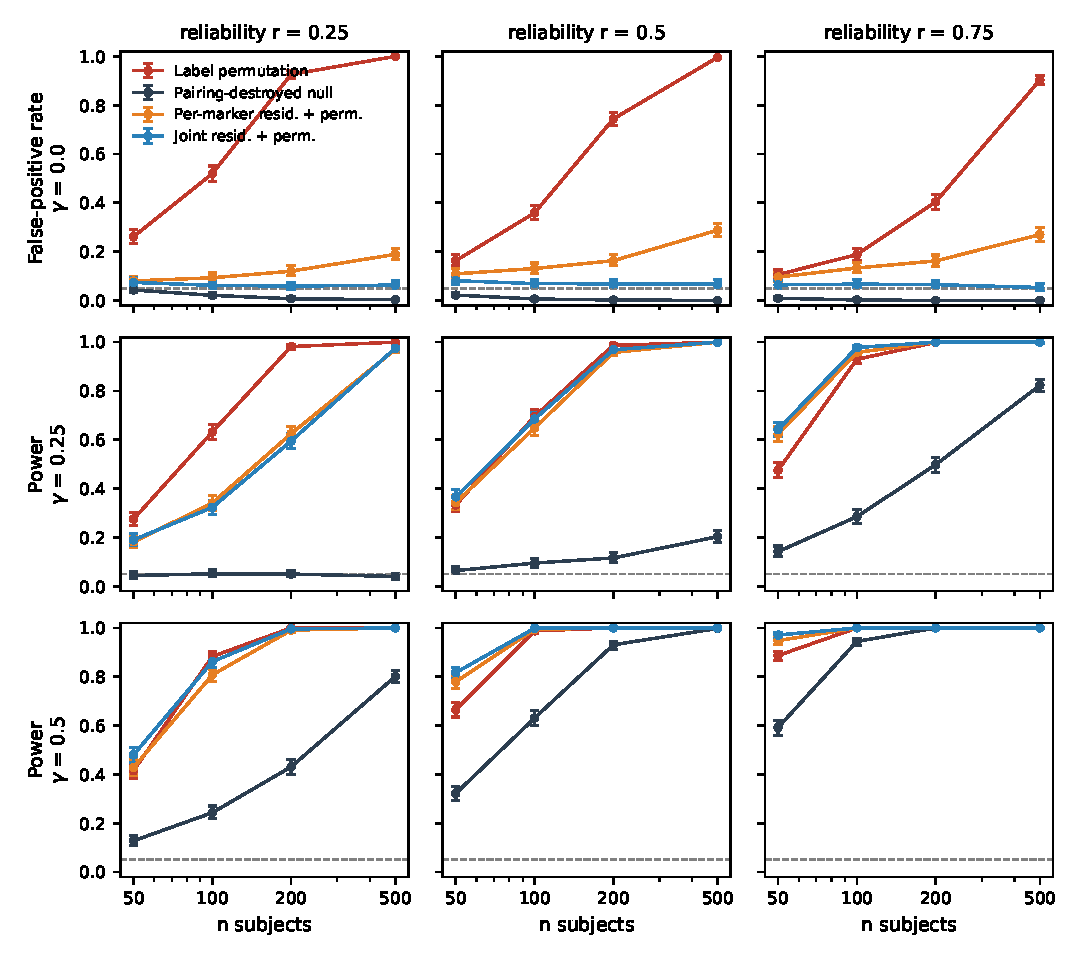
\includegraphics[width=0.82\textwidth]{figures/sim_rejection.pdf}
\caption{Rejection rate vs.\ number of subjects. Top row: false-positive rate
with no individual response ($\gamma=0$). Lower rows: power with a real,
forecastable response. Columns: reliability $r$. Dashed line: $\alpha=0.05$.
Error bars: Wilson 95\% intervals over 1{,}000 datasets.}
\label{fig:sim}
\end{figure*}

\subsection{Implication for Case 1}
The per-marker correction used in our original analysis is liberal, so
Section~\ref{sec:case1} repeats the corrected analysis with joint
residualisation. The conclusion is unchanged: the model does no better than
an unfitted scorer, and the subject-bootstrap interval spans zero. Because a
liberal test and a near-nominal test both found nothing, the null result is
not an artefact of the per-marker correction. It remains absence of evidence
at $n=71$, not evidence that preoperative profiles cannot forecast response:
the simulation shows that even joint residualisation has little power at this
sample size and reliability.

% ===========================================================================
\section{Discussion}
\label{sec:discussion}

\subsection{A checklist for small-$n$ metabolomics ML}
\begin{enumerate}
  \item If the outcome is computed from the features, do not rely on a
        label permutation. Residualise change on \emph{all} baselines inside
        each training fold, and report a pairing-destroyed null as a
        diagnostic.
  \item Refit the model inside every permutation replicate, and check that
        the observed statistic does not sit below the whole null, which
        signals a mis-specified null rather than strong evidence.
  \item Include a learn-nothing baseline and report the gap with an interval
        that resamples subjects.
  \item Audit features for exogenous compounds; report results with and
        without them.
  \item Cross-tabulate the label against every metadata column (batch, run
        order, sample-name prefix, sex) and read the collection protocol for
        each class.
  \item State in one sentence what the label physically encodes.
\end{enumerate}

\subsection{Limitations}
The empirical cases use three small public datasets, chosen because their
problems are verifiable from the published files, and they audit our own
earlier analyses rather than a sample of the literature; we make no claim
about how common these failures are. The findings concern validation
practice; they say nothing for or against the biology of obesity or diabetes.
Regression to the mean is classical statistics, and our contribution is
limited to showing how ML practice fails to detect it. The exogenous origin
of the Case~2 compounds is plausible for isopropanol and methanol, only
partial for dimethyl sulfone, and not established from the deposited data. The simulation uses Gaussian data, a linear ridge model and one outcome
rule; non-linear models and other rules may differ in degree. The
pairing-destroyed null is conservative and can miss real effects at low
reliability, so it should be a diagnostic, not the sole test. Finally, the
joint residualisation removes any \emph{true} biological dependence of change
on baseline together with the artefact; separating the two needs repeated
baseline measurements.

% ===========================================================================
\section{Conclusion}
\label{sec:conclusion}
Cross-validation, permutation tests and attribution checks are necessary but
answer narrow questions. In four of our own analyses of public data, a
standard check passed while the result was wrong: an outcome built from its
own features, putatively exogenous compounds ranked alongside endogenous
metabolites, a collection protocol equal to the label, and a label named for
something it did not measure. Each failure has a cheap, targeted control. We
recommend that small-$n$ metabolomics ML studies report these controls
alongside their headline score, and we release code that runs them.

% ===========================================================================
\section*{Data and Code Availability}
MTBLS242, MTBLS1 and MTBLS881 are public through MetaboLights \cite{haug2020};
the datasets are not redistributed. The simulation, the Case~2, 3 and 4
analyses, intermediate results and the pre-registration file for the MTBLS881
replication are in \url{https://github.com/Calvinkub/validated-yet-wrong}
(tag \texttt{paper-v1}) \todo{repository returns 404 (private) as of
18 Oct.\ 2026: make it public and create the tag}. Each experiment folder
contains a \texttt{RESULTS.md} listing every reported number with its script,
random seed and command. The simulation runs with
\texttt{python simulation/sim\_pairing\_null.py} and takes about 11 minutes on
8 cores; \texttt{--check} runs the pure-noise sanity test. The original
analyses audited in Cases~2--4 are public \cite{bridge2026, roar2026}. Cases~1
and 1b import the outcome, model and control code from our earlier
\texttt{mtbls242-forecast-honest} repository \cite{honest2026}, which must be
obtained separately \todo{commit \texttt{637a58e} is not on GitHub: push it
and add the URL, or state that the code is available on request}.

\section*{Acknowledgment}
\todo{Funding, advisors.}

\section*{Use of Generative AI}
The authors used Claude (Anthropic) to assist with analysis code, the
simulation, and drafting text. The authors are responsible for the content
of this paper.

% ===========================================================================
\begin{thebibliography}{00}
\bibitem{mtbls242} EMBL-EBI, ``MetaboLights study MTBLS242: Metabolomic fingerprint of severe obesity is dynamically affected by bariatric surgery in a procedure-dependent manner,'' dataset. [Online]. Available: \url{https://www.ebi.ac.uk/metabolights/MTBLS242}
\bibitem{gralka2015} E. Gralka, C. Luchinat, L. Tenori, B. Ernst, M. Thurnheer, and B. Schultes, ``Metabolomic fingerprint of severe obesity is dynamically affected by bariatric surgery in a procedure-dependent manner,'' \textit{Am. J. Clin. Nutr.}, vol. 102, no. 6, pp. 1313--1322, Dec. 2015, doi: 10.3945/ajcn.115.110536.
\bibitem{salek2007} R. M. Salek \textit{et al.}, ``A metabolomic comparison of urinary changes in type 2 diabetes in mouse, rat, and human,'' \textit{Physiol. Genomics}, vol. 29, no. 2, pp. 99--108, Apr. 2007, doi: 10.1152/physiolgenomics.00194.2006.
\bibitem{haug2020} K. Haug \textit{et al.}, ``MetaboLights: a resource evolving in response to the needs of its scientific community,'' \textit{Nucleic Acids Res.}, vol. 48, no. D1, pp. D440--D444, Jan. 2020, doi: 10.1093/nar/gkz1019.
\bibitem{oldham1962} P. D. Oldham, ``A note on the analysis of repeated measurements of the same subjects,'' \textit{J. Chronic Dis.}, vol. 15, no. 10, pp. 969--977, 1962, doi: 10.1016/0021-9681(62)90116-9.
\bibitem{tu2007} Y.-K. Tu and M. S. Gilthorpe, ``Revisiting the relation between change and initial value: a review and evaluation,'' \textit{Stat. Med.}, vol. 26, no. 2, pp. 443--457, Jan. 2007, doi: 10.1002/sim.2538.
\bibitem{barnett2005} A. G. Barnett, J. C. van der Pols, and A. J. Dobson, ``Regression to the mean: what it is and how to deal with it,'' \textit{Int. J. Epidemiol.}, vol. 34, no. 1, pp. 215--220, Feb. 2005, doi: 10.1093/ije/dyh299.
\bibitem{kapoor2023} S. Kapoor and A. Narayanan, ``Leakage and the reproducibility crisis in machine-learning-based science,'' \textit{Patterns}, vol. 4, no. 9, Art. no. 100804, Sep. 2023, doi: 10.1016/j.patter.2023.100804.
\bibitem{leek2010} J. T. Leek \textit{et al.}, ``Tackling the widespread and critical impact of batch effects in high-throughput data,'' \textit{Nat. Rev. Genet.}, vol. 11, no. 10, pp. 733--739, Oct. 2010, doi: 10.1038/nrg2825.
\bibitem{collins2024} G. S. Collins \textit{et al.}, ``TRIPOD+AI statement: updated guidance for reporting clinical prediction models that use regression or machine learning methods,'' \textit{BMJ}, vol. 385, Art. no. e078378, 2024, doi: 10.1136/bmj-2023-078378.
\bibitem{hooker2019} S. Hooker, D. Erhan, P.-J. Kindermans, and B. Kim, ``A benchmark for interpretability methods in deep neural networks,'' in \textit{Proc. Adv. Neural Inf. Process. Syst. (NeurIPS)}, vol. 32, 2019.
\bibitem{lundberg2017} S. M. Lundberg and S.-I. Lee, ``A unified approach to interpreting model predictions,'' in \textit{Proc. Adv. Neural Inf. Process. Syst. (NeurIPS)}, vol. 30, 2017.
\bibitem{ojala2010} M. Ojala and G. C. Garriga, ``Permutation tests for studying classifier performance,'' \textit{J. Mach. Learn. Res.}, vol. 11, pp. 1833--1863, 2010.
\bibitem{chen2016} T. Chen and C. Guestrin, ``XGBoost: A scalable tree boosting system,'' in \textit{Proc. 22nd ACM SIGKDD Int. Conf. Knowl. Discov. Data Min.}, 2016, pp. 785--794, doi: 10.1145/2939672.2939785.
\bibitem{archie1981} J. P. Archie, ``Mathematic coupling of data: a common source of error,'' \textit{Ann. Surg.}, vol. 193, no. 3, pp. 296--303, Mar. 1981, doi: 10.1097/00000658-198103000-00008.
\bibitem{vickers2001} A. J. Vickers and D. G. Altman, ``Analysing controlled trials with baseline and follow up measurements,'' \textit{BMJ}, vol. 323, no. 7321, pp. 1123--1124, 2001, doi: 10.1136/bmj.323.7321.1123.
\bibitem{glymour2005} M. M. Glymour, J. Weuve, L. F. Berkman, I. Kawachi, and J. M. Robins, ``When is baseline adjustment useful in analyses of change? An example with education and cognitive change,'' \textit{Am. J. Epidemiol.}, vol. 162, no. 3, pp. 267--278, Aug. 2005, doi: 10.1093/aje/kwi187.
\bibitem{teahan2006} O. Teahan \textit{et al.}, ``Impact of analytical bias in metabonomic studies of human blood serum and plasma,'' \textit{Anal. Chem.}, vol. 78, no. 13, pp. 4307--4318, Jul. 2006, doi: 10.1021/ac051972y.
\bibitem{han2022} W. Han and L. Li, ``Evaluating and minimizing batch effects in metabolomics,'' \textit{Mass Spectrom. Rev.}, vol. 41, no. 3, pp. 421--442, May 2022, doi: 10.1002/mas.21672.
\bibitem{adebayo2018} J. Adebayo, J. Gilmer, M. Muelly, I. Goodfellow, M. Hardt, and B. Kim, ``Sanity checks for saliency maps,'' in \textit{Proc. Adv. Neural Inf. Process. Syst. (NeurIPS)}, vol. 31, 2018.
\bibitem{kumar2020} I. E. Kumar, S. Venkatasubramanian, C. Scheidegger, and S. Friedler, ``Problems with Shapley-value-based explanations as feature importance measures,'' in \textit{Proc. 37th Int. Conf. Mach. Learn. (ICML)}, PMLR vol. 119, 2020, pp. 5491--5500.
\bibitem{vandersar2015} S. A. van der Sar \textit{et al.}, ``Ethanol contamination of cerebrospinal fluid during standardized sampling and its effect on $^1$H-NMR metabolomics,'' \textit{Anal. Bioanal. Chem.}, vol. 407, no. 16, pp. 4835--4839, Jun. 2015, doi: 10.1007/s00216-015-8663-9.
\bibitem{bernini2011} P. Bernini, I. Bertini, C. Luchinat, P. Nincheri, S. Staderini, and P. Turano, ``Standard operating procedures for pre-analytical handling of blood and urine for metabolomic studies and biobanks,'' \textit{J. Biomol. NMR}, vol. 49, no. 3--4, pp. 231--243, 2011, doi: 10.1007/s10858-011-9489-1.
\bibitem{westerhuis2008} J. A. Westerhuis \textit{et al.}, ``Assessment of PLSDA cross validation,'' \textit{Metabolomics}, vol. 4, no. 1, pp. 81--89, 2008, doi: 10.1007/s11306-007-0099-6.
\bibitem{varma2006} S. Varma and R. Simon, ``Bias in error estimation when using cross-validation for model selection,'' \textit{BMC Bioinformatics}, vol. 7, Art. no. 91, 2006, doi: 10.1186/1471-2105-7-91.
\bibitem{varoquaux2018} G. Varoquaux, ``Cross-validation failure: Small sample sizes lead to large error bars,'' \textit{NeuroImage}, vol. 180, pp. 68--77, 2018, doi: 10.1016/j.neuroimage.2017.06.061.
\bibitem{broadhurst2006} D. I. Broadhurst and D. B. Kell, ``Statistical strategies for avoiding false discoveries in metabolomics and related experiments,'' \textit{Metabolomics}, vol. 2, no. 4, pp. 171--196, 2006, doi: 10.1007/s11306-006-0037-z.
\bibitem{engelke2005} U. F. H. Engelke \textit{et al.}, ``Dimethyl sulfone in human cerebrospinal fluid and blood plasma confirmed by one-dimensional $^1$H and two-dimensional $^1$H-$^{13}$C NMR,'' \textit{NMR Biomed.}, vol. 18, no. 5, pp. 331--336, Aug. 2005, doi: 10.1002/nbm.966.
\bibitem{bridge2026} K. C. Shomwiwat, ``Bridge\_ai\_summit\_nmr\_2026,'' GitHub repository, commits \texttt{17e18df} (Case~4) and \texttt{0088e38} (Case~3), 2026. [Online]. Available: \url{https://github.com/Calvinkub/Bridge_ai_summit_nmr_2026}
\bibitem{roar2026} C. Orrudee, ``ROAR,'' GitHub repository, commit \texttt{f220cd2} (Case~2), 2026. [Online]. Available: \url{https://github.com/Chaiporn2005/ROAR}
\bibitem{honest2026} ``mtbls242-forecast-honest,'' code repository, branch \texttt{honest-evaluation}, commit \texttt{637a58e} (Cases~1 and 1b), 2026. \todo{add author and URL once public}
\bibitem{maltesen2020} R. G. Maltesen, R. Wimmer, and B. S. Rasmussen, ``A longitudinal serum NMR-based metabolomics dataset of ischemia-reperfusion injury in adult cardiac surgery,'' \textit{Sci. Data}, vol. 7, Art. no. 198, 2020, doi: 10.1038/s41597-020-0545-0.
\end{thebibliography}

\end{document}
